\def\Titel{Die Gedanken sind frei}
\def\Interpret{Deutsches Volkslied}
\def\Referenz{Möglicher Querverweis auf ein gebräuchliches Liederbuch deiner Wahl}

% hier entweder \LiedSetup() oder \GeistlichSetup{} wenn es im Kuratenverzeichnis auftauchen soll
\LiedSetup{}

\begin{guitarMagic}
	\begin{enumerate}

        \item Die Ge[A]danken sind frei, wer [E7]kann sie er[A]raten? \\
        Sie fliehen vorbei wie [E7]nächtliche [A]Schatten.\\
        Kein [E]Mensch kann sie [A]wissen, kein [E]Jäger er[A]schießen
        mit [D]Pulver und [A]Blei.\\
        Die Ge[E]danken sind [A]frei!

        \item Ich [A]denke, was ich will und [E]was mich be[A]glücket,\\
        doch alles in der Still’
        und [E]wie es sich [A]schicket.\\
        Mein [E]Wunsch und Be[A]gehren
        kann [E]niemand ver[A]wehren,
        es [D]bleibet da[A]bei:\\
        Die Ge[E]danken sind [A]frei!
        % So wird ein Seitenumbruch mit dem "auf der nächsten Seite gehts weiter" eingefügt
        \liedweiter{}

        \item Und [A]sperrt man mich ein
        im [E7]finsteren [A]Kerker,\\
        das alles sind rein
        ver[E7]gebliche [A]Werke,\\
        denn [E]meine Ge[A]danken
        zer[E]reißen die [A]Schranken
        und [D]Mauern ent[A]zwei.\\
        Die Ge[E]danken sind [A]frei!

        \item Drum [A]will ich auf immer
        den [E7]Sorgen ent[A]sagen\\
        und will mich auch nimmer
        mit [E7]Grillen mehr [A]plagen.\\
        Man [E]kann ja im [A]Herzen
        stets [E]lachen und [A]scherzen
        und [D]denken da[A]bei:\\
        Die Ge[E]danken sind [A]frei!

        \item Ich [A]liebe den Wein,
        mein [E7]Mädchen vor [A]allen,\\
        sie tut mir allein
        am [E7]besten ge[A]fallen.
        
        \liedweiter{}

        Ich [E]bin nicht al[A]leine
        bei [E]meinem Glas [A]Weine,
        mein [D]Mädchen da[A]bei.\\
        Die Ge[E]danken sind [A]frei!

    \end{enumerate}
\end{guitarMagic}

% Bilder können nicht in der guitarmagic Umgebung eingefügt werden. Das muss davor oder danach geschehen
\begin{picture}(0,0)
    \put(-5,-150){\hbox{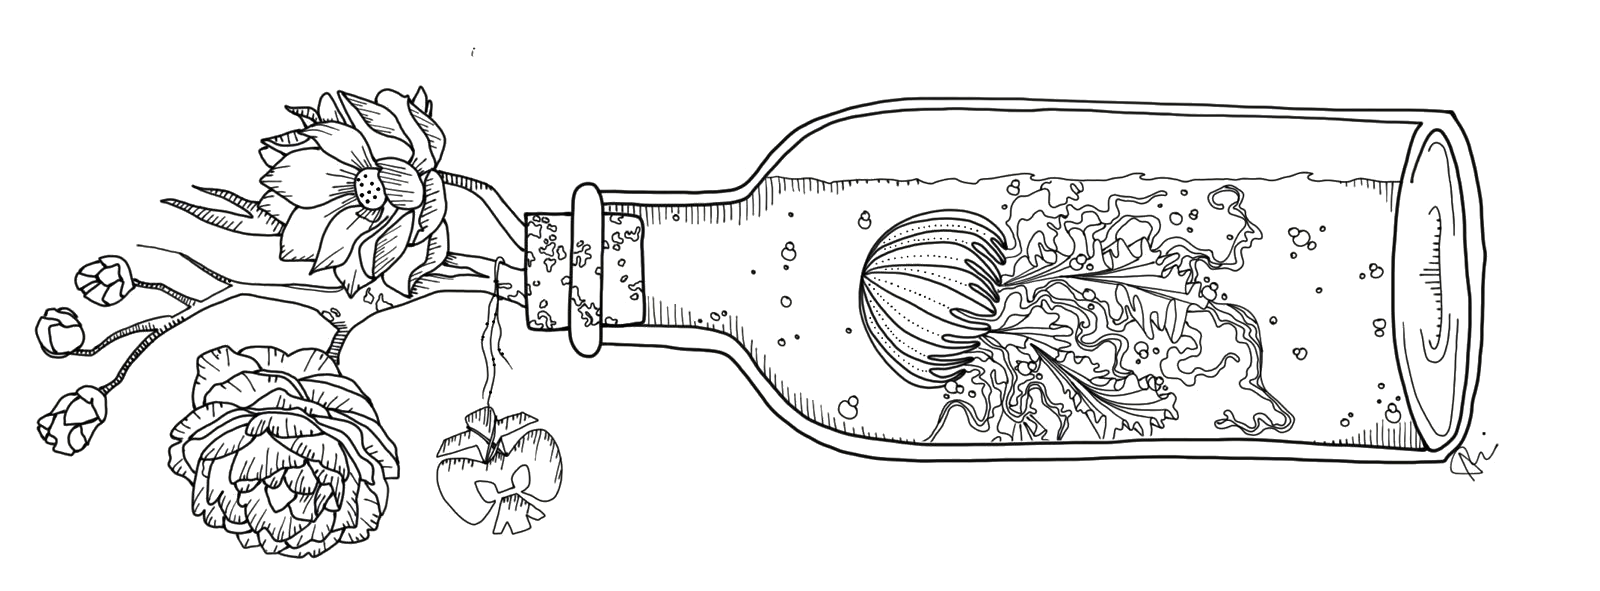
\includegraphics[scale=0.25, angle=0]{bilder/Flaschenpost.png}}}
\end{picture}

